\newcommand{\fni}{\mathscr{I^+}}
\newcommand{\Msun}{\ensuremath{\mathrm{M}_\odot}

\section{Overview of the event}

\section{Direct comparison of the data and best fit template}
\subsection{Filtering the data}
The raw GW strain seen by the LIGO detectors are recorded in a channel called GDS-CALIB-STRAIN. We use the timeseries recorded in this channel and perform a minimal set of filtering needed to visually see the GW event. We first whiten the data (i.e) apply inverse detector power spectral density (PSD) curve. Then the data is bandpassed and the harmonics of powerline frequencies are notched out using an analytical zero-pole-gain(zpk) filter. The filter is depicted in the bottom right inlay panel of figure \ref{fig:overlayGW150914}. The filter amplitude is set to 1 at 100 Hz. The data is filtered forward and backward to ensure that filtering does not introduce a phase error. The filter is acausal and is designed to introduce zero-phase offset and this can be seen in the top right inlay panel of figure \ref{fig:overlayGW150914}.

\subsection{Best fit template}

\begin{itemize}
\item Reported merger time
	\begin{itemize}
	\item L1: 1126259462.415039062 sec
    \item H1: 1126259462.422363281 sec (or 7.32msec later, corresponding to 120 samples at 16384Hz)
	\end{itemize}
\item Effective distance
	\begin{itemize}
	\item L1: 1194.9118 Mpc 
	\item H1: 970.70534 Mpc
	\end{itemize}
\item Template phase
	\begin{itemize}
	\item L1: 0.58 radians
	\item H1: -2.77 radians
	\end{itemize}
\end{itemize}

Details of the best fit template,

\begin{itemize}
\item m1=47.932518 Msun
\item m2=36.597004 Msun
\item s1=0.96167207
\item  s2=-0.8996653
\end{itemize}

This corresponds to the following ringdown parameters

\begin{itemize}
\item f=228Hz
\item Q=3.651
\end{itemize}





\begin{figure*}
\subfloat{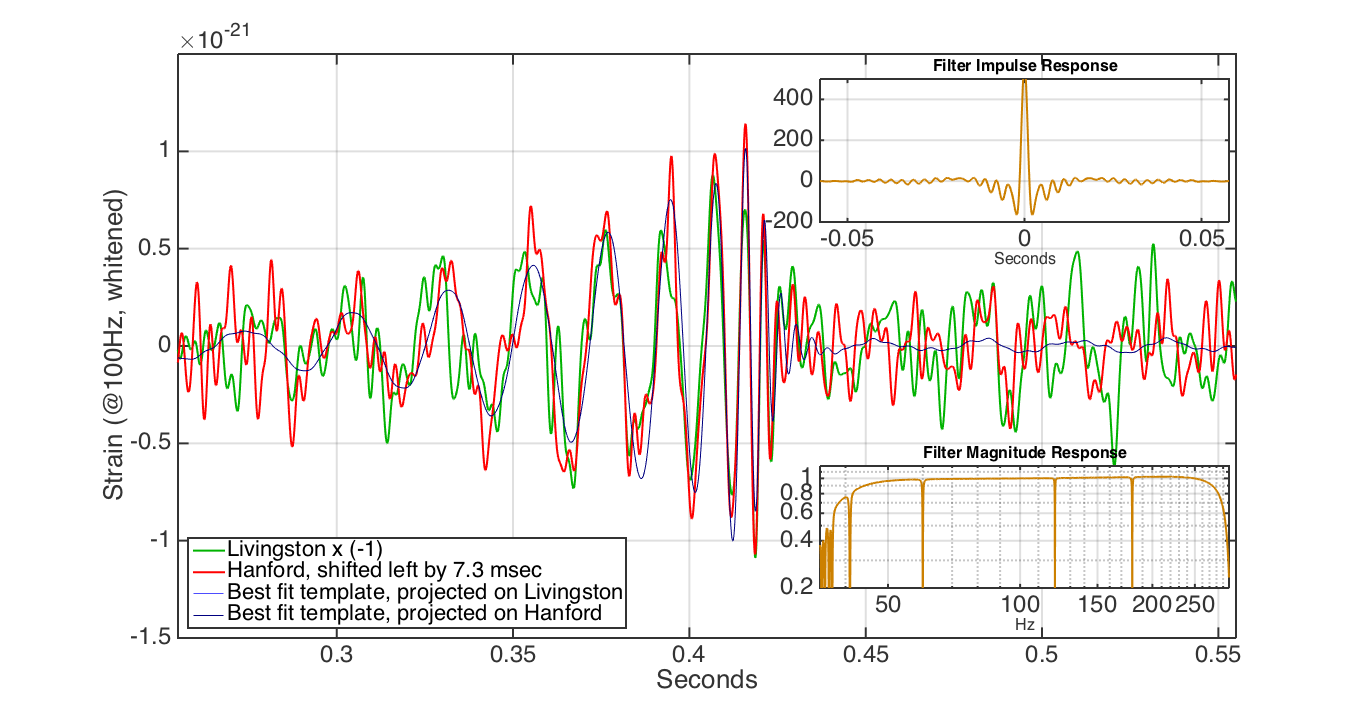
\includegraphics[width=\textwidth]{figures/overlayGW150914.png} }
\caption{Direct comparison of the detector data with the best fit template. The data from the H1 and L1 have been minimally filtered and  appropriately shifted to align with each other. The best fit template corresponding to each of the detector timeseries is overlayed on the data. The inlay panel display the details of the filters used to condition the data}
\label{fig:overlayGW150914}
\end{figure*}
}


\section{Parameters of the system}
\subsection{From properties paper}
\subsection{1606.01210}

